\section{Slackline specific training and effects to the human body}\label{2_2_slacklineTraining}

%The slacklining assistance system should mainly train and support beginners, or so called slackers, to walk on the slackline. Beyond that new skill acquisition for further training should be appropriately realised with the system. Therefore it is important to have a concrete baseline about what exercises and tips are useful for very beginners. Prior research justifies the applicability for areas like sport medicine and rehabilitation training in which such a system could be embedded. It could be used as an alternative to classical balance training because the slackline itself varies largely in space and the user has to use the whole body to balance her swift on the line~\cite{Pfusterschmied2013-yy}. Donath et al.~\cite{Donath2016-rt} found in his meta-analysis significant improvements in the postural control after slackline training, which indicates the efficacy of this training method on the human body.
As in other sport activities it is important to have a concrete baseline about what exercises and tips are useful for very beginners. Mainly to have a good knowledge of the basics, which results in a faster learning process, but also to prevent injuries from the beginning. In the following several slackline learning techniques will be discussed, which can then be implemented in the assistance system. Prior research indicates the applicability of slackline training for areas like sport medicine and rehabilitation training. It shows why slacklining could be used as an alternative to classical balance training and how the body swift affect these. Donath et al.~\cite{Donath2016-rt} found in his meta-analysis significant improvements in the postural control after slackline training, which indicates the efficacy of this training method. This subsection shows several application scenarios in which a slackline can be implemented and improve the training effect.

\subsection{Exercises during slackline training}\label{2_1_1_slacklineTraining}

For beginners it is difficult to walk or even stay on a slackline. The uncontrollable swift of the narrow line result in unfamiliar movements that cannot be handled at the very beginning. Therefore they should learn to concentrate, build up motoric basics and trust into the line, as well as manage their body behaviour.

Thoman~\cite{Thomann2013-aa} differentiate two basic methods for the learning process on a slackline. Teaching a slackline beginner, further called slacker, without any help or with systematic external assistance. The investigation of Kroiß~\cite{Kroiss2007-ab} resulted in no significant difference between both methods. But there is a trend regarding providing methodological aid, like human support or physical objects as nordic walking sticks or a bar, can help to improve the learning effect (Figure \ref{fig:supportiveExercises}). Therefore it is a good advise for beginners to learn the fundamentals of standing and walking on the slackline to build up a groundwork. Several basic techniques and tips are useful to support her in this way. For example focusing on a specific point, stretching out the arm, raising the hands over the shoulder level, turning the palms to the top, going slightly in the knees, have the feet straight with the line, and so on~\cite{Kleindl2011-bl, Kroiss2007-ab}.

\begin{figure}[htb]
	\centering
	\begin{minipage}[t]{0.23\linewidth}
		\centering
		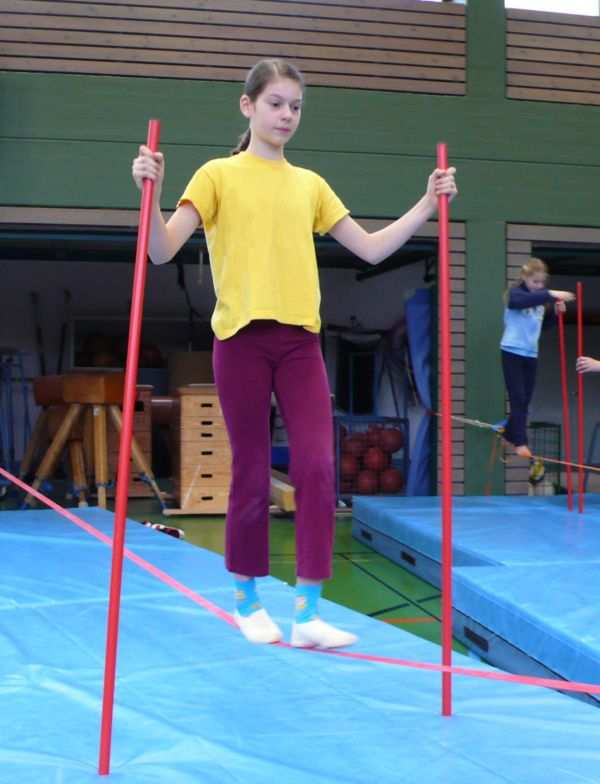
\includegraphics[width=1\linewidth]{Pictures/slacklineHelpSticks}
		\subcaption{Stick support}
		\label{fig:slacklineHelpSticks}
	\end{minipage}
	\hfill
	\begin{minipage}[t]{0.37\linewidth}
		\centering
		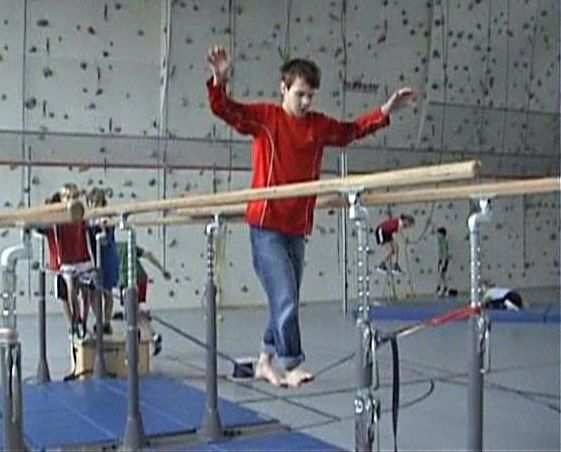
\includegraphics[width=1\linewidth]{Pictures/slacklineHelpBar}
		\subcaption{Between bars}
		\label{fig:slacklineHelpBar}
	\end{minipage}
	\hfill
	\begin{minipage}[t]{0.3\linewidth}
		\centering
		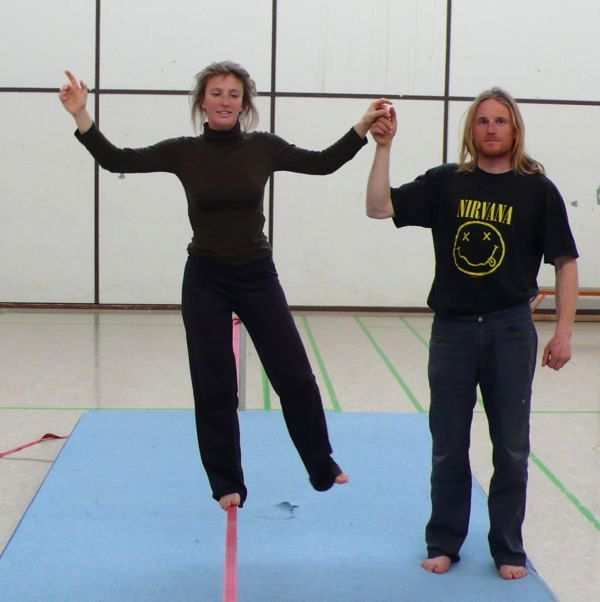
\includegraphics[width=1\linewidth]{Pictures/slacklineHelpHuman}
		\subcaption{Human support}
		\label{fig:slacklineHelpHuman}
	\end{minipage}
	\caption{Supportive exercises~\cite{Kroiss2007-ab}}
	\label{fig:supportiveExercises}
\end{figure}

With further progress, the external help, if given, should be reduced. The slacker can now try to stay and walk on the line on her own. It is recommended to begin with the practice of a basic start, to stay with both feet, and one feet on the slackline since these are basic techniques (Figure \ref{fig:basicExercises}). Staying with both feet seems easier in the beginning but only the hips and hands can be used for balancing. With just one feet on the line, the slacker can use the other one as an additional extremity for balancing purposes.
%For this one feet stays on the line and the other nearby on the ground. With a little swing the bodie's center of gravity should be brought over the slackline. A fundamental technique is to stay on one and both feet.

\begin{figure}[htb]
	\centering
	\begin{minipage}[t]{0.30\linewidth}
		\centering
		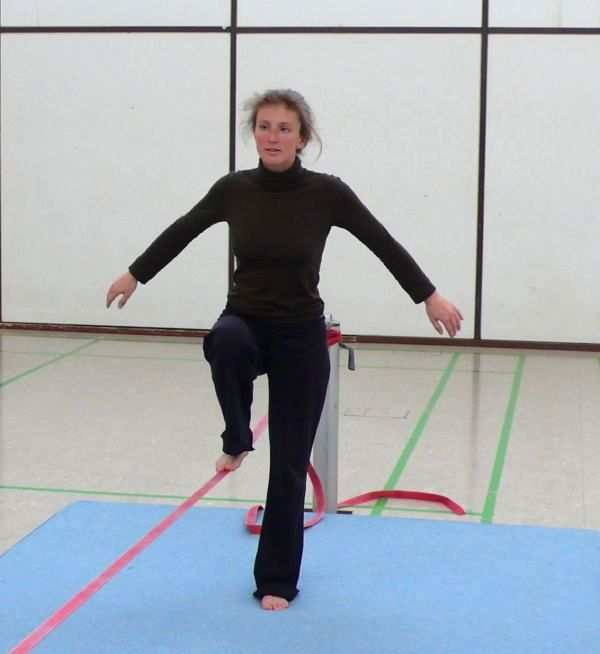
\includegraphics[width=1\linewidth]{Pictures/slacklineBasicStart}
		\subcaption{Basic start}
		\label{fig:slacklineBasicStart}
	\end{minipage}
	\hfill
	\begin{minipage}[t]{0.20\linewidth}
		\centering
		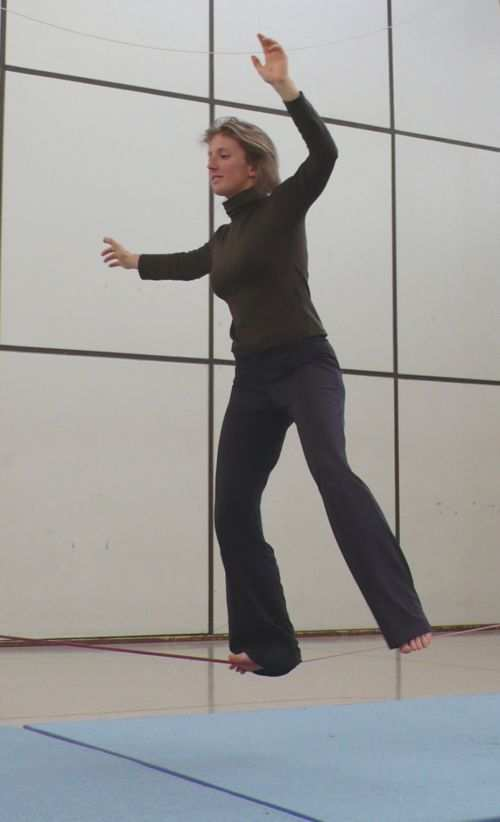
\includegraphics[width=1\linewidth]{Pictures/slacklineBasicOneFeet}
		\subcaption{One feet}
		\label{fig:slacklineBasicOneFeet}
	\end{minipage}
	\hfill
	\begin{minipage}[t]{0.33\linewidth}
		\centering
		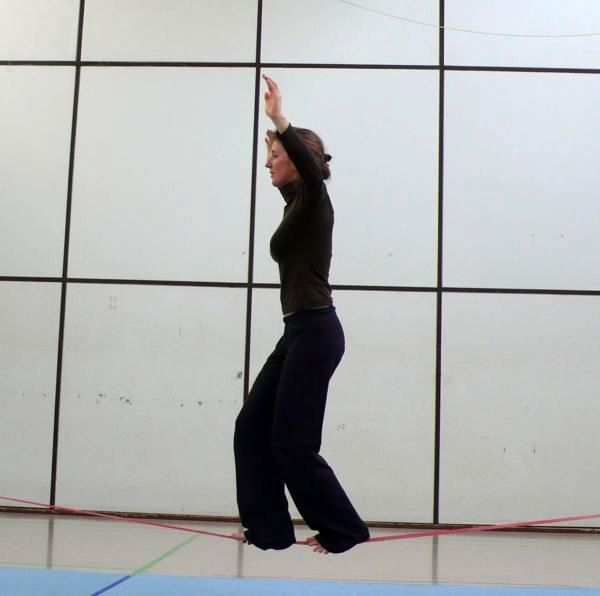
\includegraphics[width=1\linewidth]{Pictures/slacklineBasicBothFeet}
		\subcaption{Both feet}
		\label{fig:slacklineBasicBothFeet}
	\end{minipage}
	\caption{Basic exercises~\cite{Kroiss2007-ab}}
	\label{fig:basicExercises}
\end{figure}

Advanced training should be practiced in a more dynamical way~\cite{Thomann2013-aa}. Like seen in several research works~\cite{Donath2013-kk, Donath2016-gm, Granacher2010-ow, Keller2012-xh, Pfusterschmied2013-yy} this can be from crossover start (Figure \ref{fig:slacklineAdvancedCrossoverStart}), turning on the line, hands on hips or behind the back (Figure \ref{fig:slacklineAdvancedHandsBehindBack}), walk sidewards or backwards up to catch and pass a pall, kicking a football, bouncing a basketball, or a kneel down on the slackline (Figure \ref{fig:slacklineAdvancedDropknee}).

\begin{figure}[htb]
	\centering
	\begin{minipage}[t]{0.28\linewidth}
		\centering
		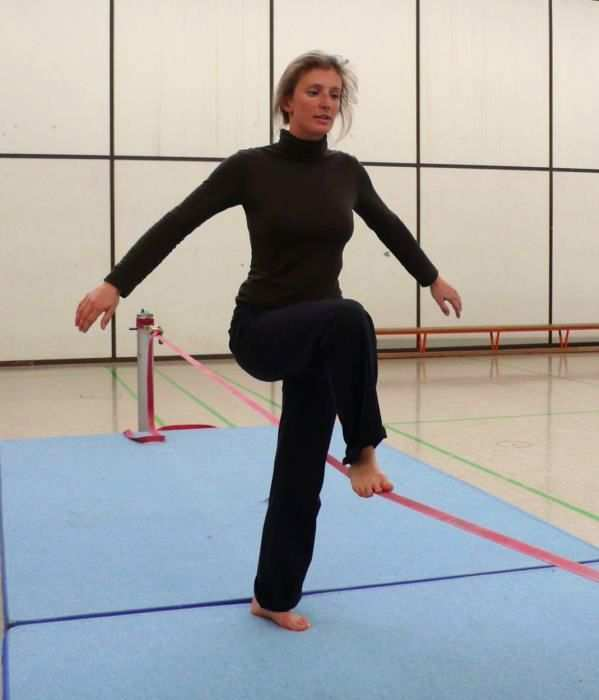
\includegraphics[width=1\linewidth]{Pictures/slacklineAdvancedCrossoverStart}
		\subcaption{Crossover start}
		\label{fig:slacklineAdvancedCrossoverStart}
	\end{minipage}	
	\hfill
	\begin{minipage}[t]{0.3\linewidth}
		\centering
		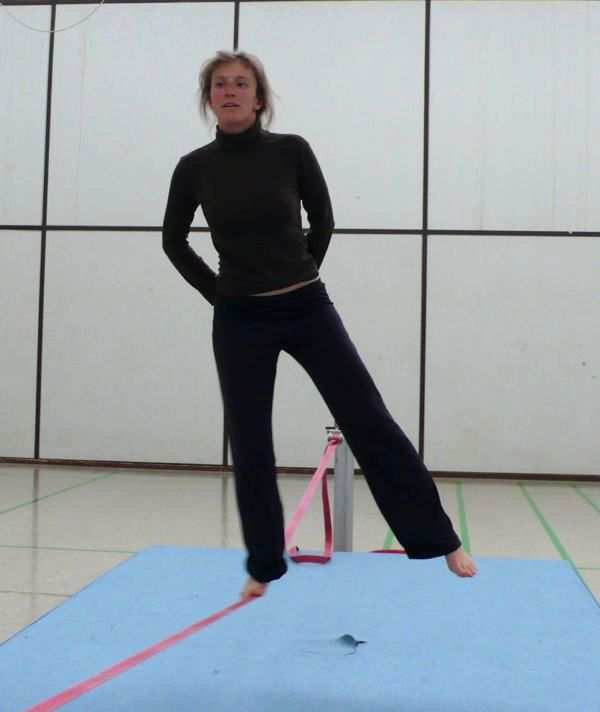
\includegraphics[width=0.9\linewidth]{Pictures/slacklineAdvancedHandsBehindBack}
		\subcaption{Hands behind back}
		\label{fig:slacklineAdvancedHandsBehindBack}
	\end{minipage}	
	\hfill
	\begin{minipage}[t]{0.38\linewidth}
		\centering
		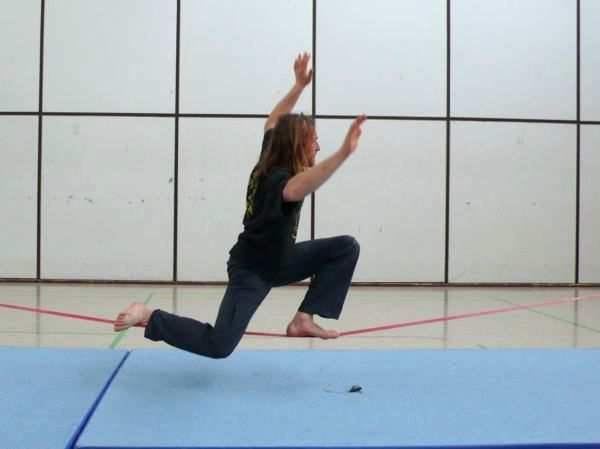
\includegraphics[width=1\linewidth]{Pictures/slacklineAdvancedDropknee}
		\subcaption{Dropknee}
		\label{fig:slacklineAdvancedDropknee}
	\end{minipage}	
	\caption{Advanced techniques~\cite{Kroiss2007-ab}}
	\label{fig:advancedExercises}
\end{figure}

Additional cognitive load is caused by unfamiliar exercises and simultaneous balancing on the line. This conjunction can lead to impairments. Even more difficult exercises can be carried out in further sessions like standing up from a sitting position, juggling, two people on the same line, reading a newspaper, closing eyes while balancing, vertical jumps, or rope skipping. Due to the higher difficulty of constraints, it results in a more unstable movement of the line.

Changes directly on the slackline itself, like varying the tension and length, have also an influence on the stability of the human body on the line~\cite{Keller2012-xh, Pfusterschmied2013-yy, Pfusterschmied2013-kq}. A short and tight line results in a relatively small vibrating area, where the slacker has to outbalance short unpredictable movements on point. Given a longer and loose line, it results in a more swinging behaviour that she has to counteract~\cite{Kroiss2007-ab}.
 
The slacklining assistance system should mainly train and support slacker to walk on the slackline. With those approaches in mind a foundation is set to build helpful exercises for the system. Because the focus relies especially on beginners, this information serves as an inspiration for supporting them with effective and efficient methods. Now is the question, what effect has slackline on the human body and where can it be applied? This is part of the next subsection.

\subsection{Slackline specific training effects and application scenarios}

Donath et al.~\cite{Donath2013-kk} elaborated the effects of slackline training on regular balancing, jump performance, and muscle activity with young children in school sport. The slackline specific balance has improved. Also the dynamic sway and muscle activity for the lower limb is reduced. But there were no effects regarding jump performance. The children enjoyed the slackline training. In comparison to classical balance training it can be more fun for the children and at the same time an effective training method.

Another study of Donath et al.~\cite{Donath2016-gm} investigated slackline training with seniors from an age between 59 to 69 to measure effects on slackline specific balance and neuromuscular performance. They found significant differences between pre- and posttests during all slackline stance conditions. In addition the trunk and limb muscle activity were reduced after the training phase. With this in mind slacklining can be provided as an alternative balance training method for seniors. Regular balance training can help to reduce the fall risk, which can be an useful therapy for seniors when keeping in mind that 30\% of seniors suffer from fall injuries once a year.

Keller et al.~\cite{Keller2012-xh} examined the improvement of the postural control regarding the Hoffmann-Reflex after slackline training and whether adaptations can be found regarding classical balance training. The H-Reflex (Hoffmann-Reflex) is used to assess and quantify stretch-reflex responses due to electrical stimulation. The measurements show that these were significantly reduced as well as slackline specific balance were improved. Therefore slackline training and classical balance training have at least similar effects on the postural control.

Pfusterschmied et al.~\cite{Pfusterschmied2013-yy} found significant effects regarding stable stance after slackline training and even more effects were found for perturbed leg stance. This is because slacklining is a high dynamic movement activity and there is more need of regaining equilibrium as in perturbed stance than for maintaining balance as in a stable leg stance condition. The velocity in medio-lateral and anterior-posterior center of gravity, knee and hip joint is reduced as well as the range motion in knee and hip joint. No changes in medio lateral direction for the stable surface or joint kinematics for both have been found.

Another study of Pfusterschmied et al.~\cite{Pfusterschmied2013-kq} shows effects on lower limb joint motion and muscle activation. They found a decrease in platform velocity and improvements in corrective action in the knee joint. Also enhanced activation of the muscle activity in rectus femoris (upper leg) was measured.

Granacher et al.~\cite{Granacher2010-ow} investigated the impact of slackline training for balance and strength promotion and found contradictory results compared with the studies described above. Static and dynamic postural control were analysed as well as the isometric and dynamic muscle strength. There were no effects regarding the postural control, maximal torque, and jumping height. The results can be explained due to the assessment of other recorded variables, usage of different methods for analysing the data, and the relatively short slackline training time than in other studies~\cite{Pfusterschmied2013-yy}. Therefore this study can be seen as an exceptional case.

Those investigations show that slacklining is indeed an effective method for improving the postural control. Hence many application scenarios can be thought of to implement a slacklining assistance system. For example it can be used as a training approach in school sport, preventative activity for seniors, and rehabilitation alternative. Furthermore it can be used as a supportive training method for athletes in sport activities like skiing or skating, that require a good body balance. Interactive technologies can be used to support training in such scenarios. The next section provides an overview about state of the art technologies, compares them, and show several implementations in balance scenarios.